\documentclass{article}
\pagenumbering{arabic} 
\usepackage{graphicx}
\usepackage[a4paper, portrait, total={6.5in, 9.6in}]{geometry}
\graphicspath{{./images/}}
\newcommand\tab[1][1cm]{\hspace*{#1}}

\usepackage{hyperref}
\hypersetup
{
	colorlinks=true,
	linkcolor=blue,
	filecolor=magenta,      
	urlcolor=cyan,
}
\urlstyle{same}

\usepackage{enumitem}
\setlist{nosep}

\begin{document}
	
	\begin{center}
		\huge\textbf{Chirag Shah}			
	\end{center}
	
	\hrulefill
	
	\noindent \parbox[t]{0.7\linewidth}
	{
		16-Marina House, \\ 5-Sir V.T Marg, \\ Opp Liberty Cinema,\\ Mumbai 400 020 \\ Maharashtra
	}	 
	\vspace{1cm}
	\parbox[t]{0.45\linewidth}
	{
		Contact: 9769168825 \\ chirags1998@gmail.com \\		
		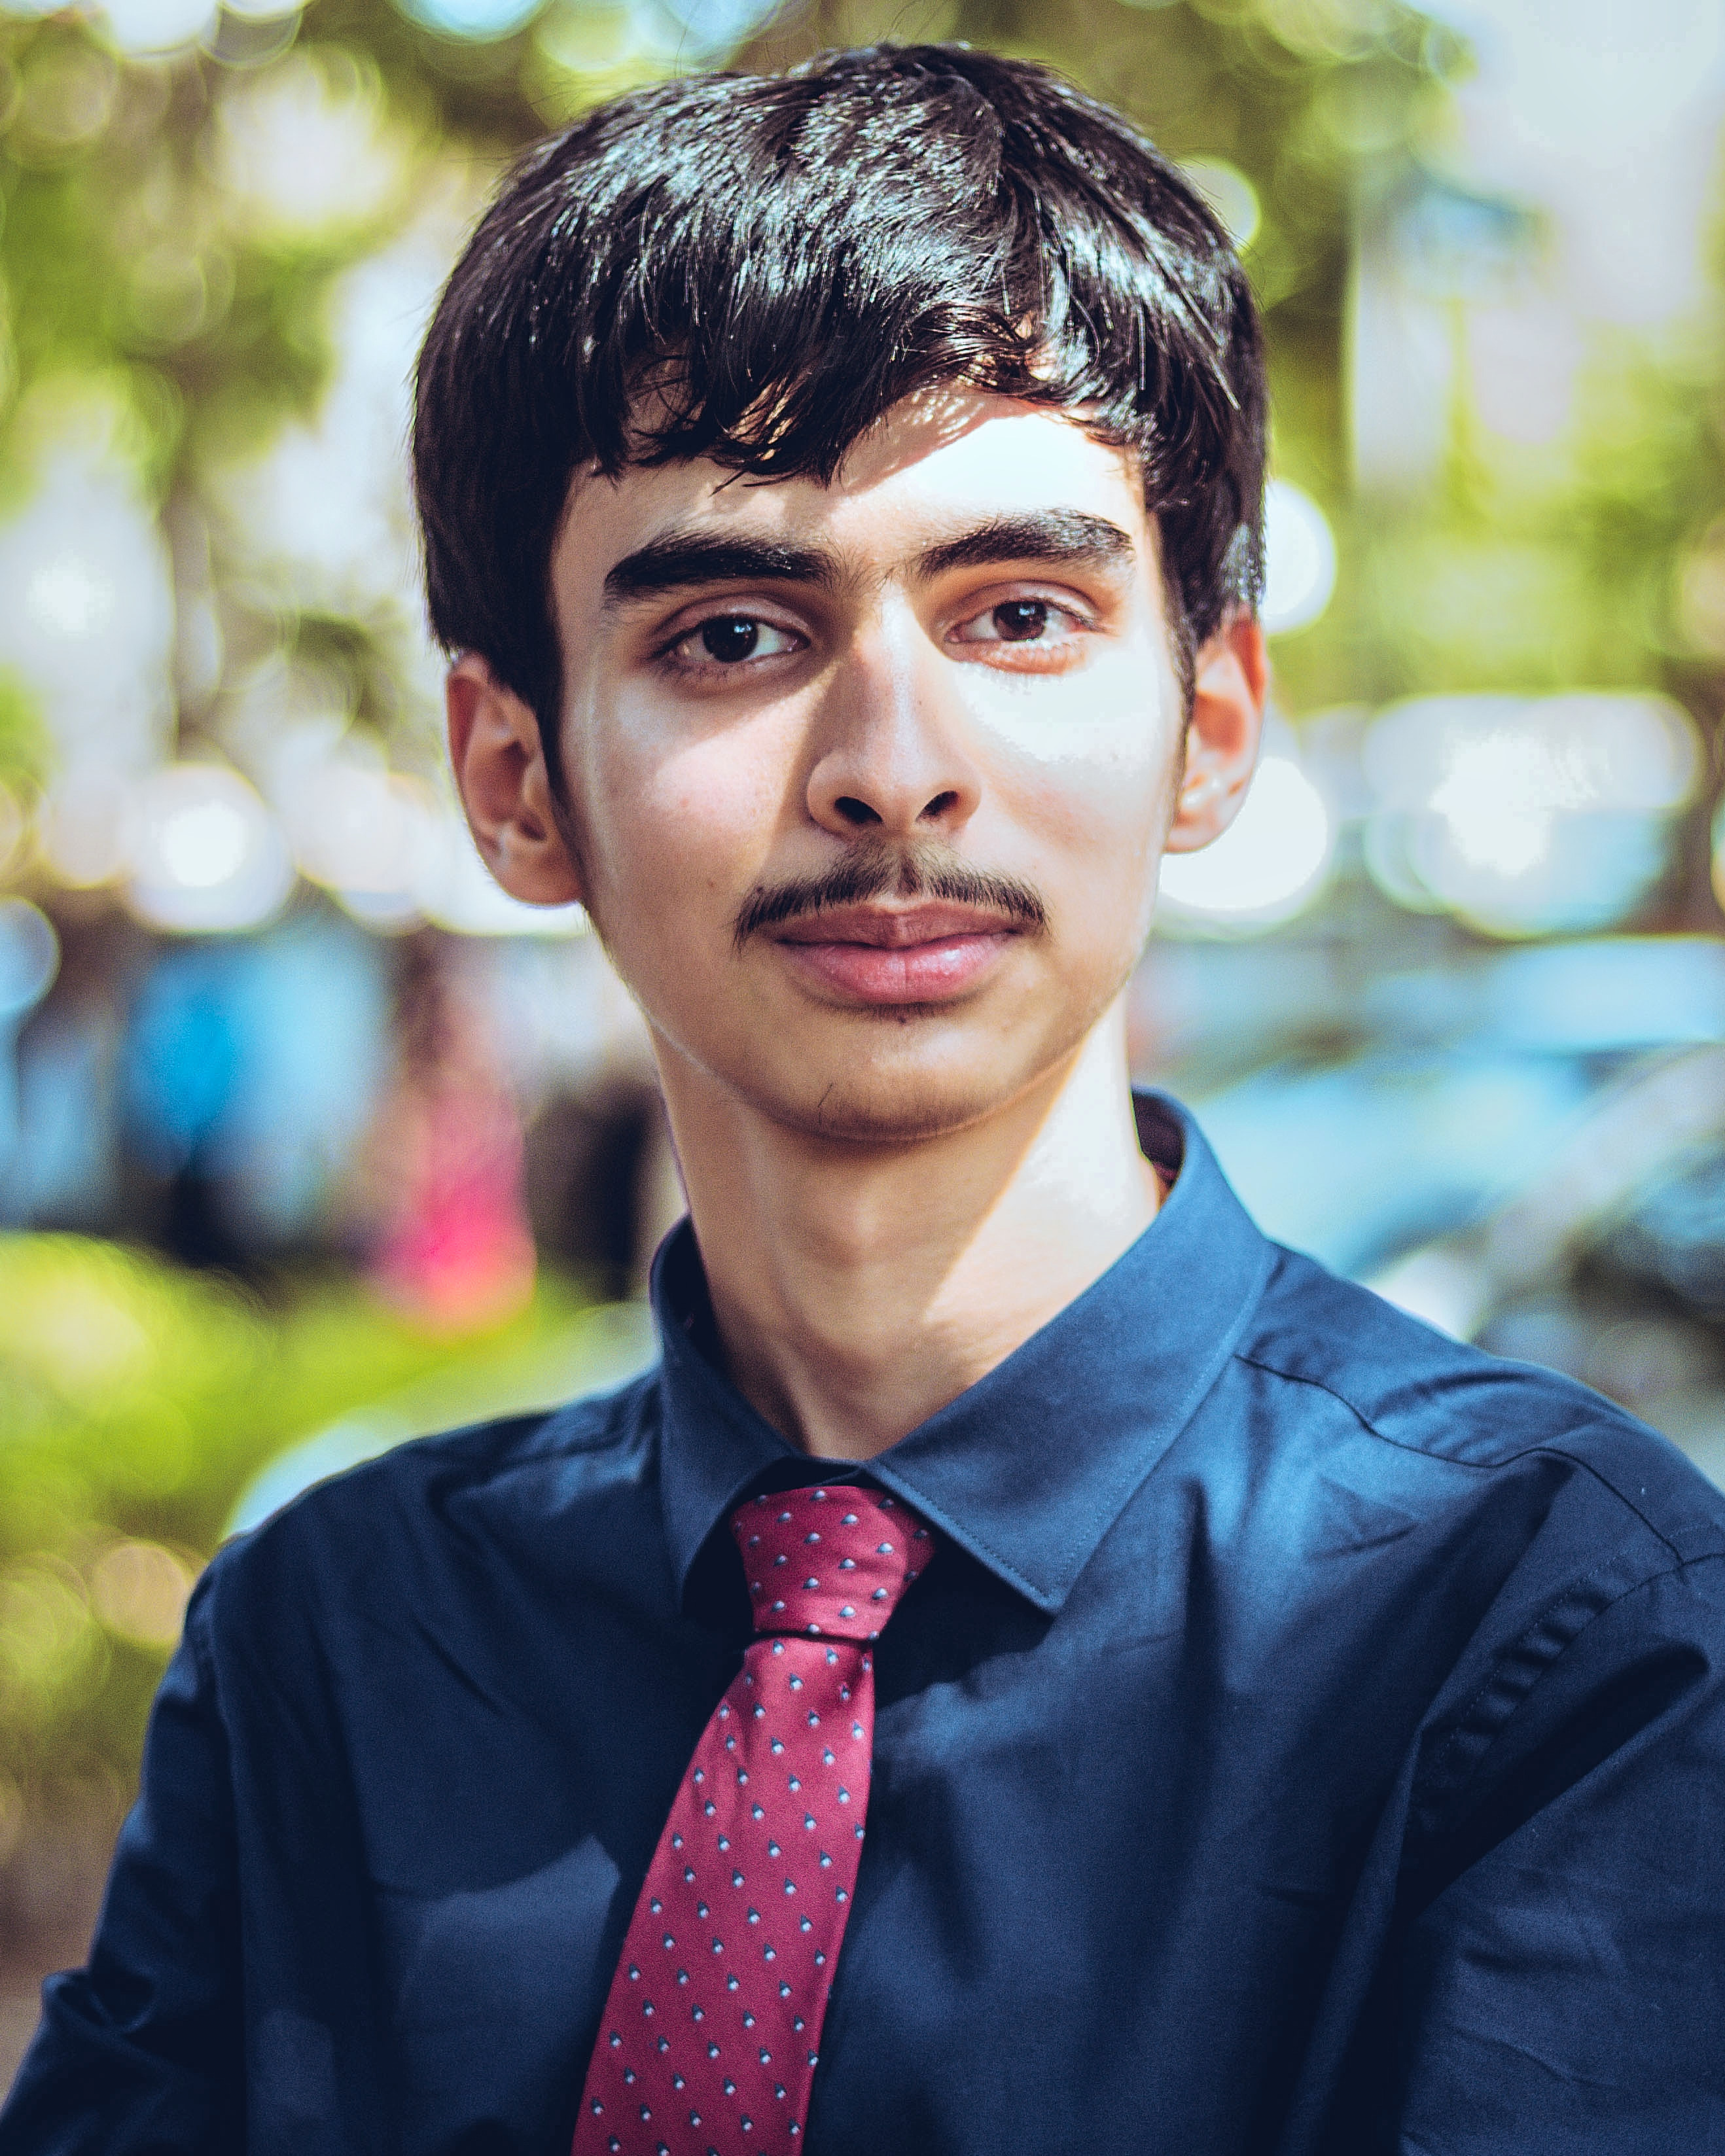
\includegraphics[scale =.1]{photo.jpg}
	}

	\section*{Career Objective}
	To work as a system/product design engineer in the electronics industry where I can develop and apply my hardware and software skills

	\section*{Education}
	\begin{tabular}{|c|c|c|c|c|}
		\hline
		Degree & College/School & University & Passing Year & Pass \% \\
		\hline
		SSC & St Xaviers High School, Fort & Maharashtra State Board  & 2013 & 87.5\\
		\hline
		HSC & PACE Junior Science College, Dadar & Maharashtra State Board & 2015 & 82.31\\
		\hline
	\end{tabular}

	\section*{Projects and Competitions}
	\begin{enumerate}%[noitemsep]
		%\setlength\itemsep{-.1em}
		
		\item My project \textbf{DIY Timelapse Dolly} was featured and won the first prize in \textbf{The Raspberry Pi contest 2016} contest on Instructables.com\\
		\url{www.instructables.com/id/DIY-Time-Lapse-Dolly-1/}
		\item Member of the team which was selected as one of 5 finalists out of 162 teams in the “Launch a Module” theme and were placed at 1st position in the theme\\
		\url{http://eycgen.e-yantra.org/index.php/validate/fff9370353355910a5556b2d87c8e4b04f50a00d}
		\item Won Second prize in Troubleshooting Competition organized by Department of Electronics Engineering held at SPIT Mumbai from 29th/Sep /2016 to 17th/Oct/2016
	\end{enumerate}

	\section*{Training and Internship}
	\begin{itemize}
		\item[$\bullet$] 3 weeks summer training program on Embedded Systems System Design held from 13/June/2016 to 8/July/2016 at SPIT College Mumbai
		\item[$\bullet$] 2 days workshop on MSP-FPGA Software and Hardware co-design conducted on 16th and 18th Sep 2016 at SPIT, Mumbai
	\end{itemize}

	\section*{Research Publications}
	\begin{enumerate}
		\item None
	\end{enumerate}

	\section*{Technical Skills}
		\begin{itemize}
			\item[$\bullet$] Embedded C programming
			\begin{itemize}
				\item[$\bullet$] ATmega2560-FireBird V
				\item[$\bullet$] ESP-8266
				\item[$\bullet$] ATmege8535 dev-board
				\item[$\bullet$] Arduino
			\end{itemize}
			\item[$\bullet$] SMD soldering
			\item[$\bullet$] Basic PCB designing and fabrication
			\item[$\bullet$] Basic FPGA programming - Atlys Spartan-6 FPGA Trainer Board
		\end{itemize}
	
	\section*{Soft Skills}
		\begin{enumerate}
			\item Patient and persistent in my projects
			\item Good analytical and problem solving solving skills
			\item Ready to adapt as needed
			%\item Good communication skills
		\end{enumerate}	
	
\end{document}